\documentclass[tikz,border=10pt]{standalone}
\usepackage{tikz}
\usepackage{amssymb}
\usetikzlibrary{shapes.geometric, arrows.meta, positioning, fit, backgrounds, calc}

\tikzset{
  startstop/.style={rectangle, rounded corners=22pt,
    minimum width=3.2cm, minimum height=1cm,
    text centered, draw=black!40, fill=gray!15,
    font=\small\bfseries},
  process/.style={rectangle, rounded corners=6pt,
    minimum width=5.5cm, minimum height=1.4cm,
    text centered, draw=black!40, fill=teal!12,
    font=\small\bfseries, align=center},
  decision/.style={rectangle, rounded corners=6pt,
    minimum width=5.5cm, minimum height=1.4cm,
    text centered, draw=black!40, fill=orange!18,
    font=\small\bfseries, align=center},
  action/.style={rectangle, rounded corners=6pt,
    minimum width=5.5cm, minimum height=1.4cm,
    text centered, draw=black!40, fill=red!12,
    font=\small\bfseries, align=center},
  sidenote/.style={rectangle, rounded corners=4pt,
    minimum width=1.6cm, minimum height=1.1cm,
    text centered, draw=black!30, fill=blue!12,
    font=\scriptsize\bfseries, align=center},
  sideaction/.style={rectangle, rounded corners=4pt,
    minimum width=2.2cm, minimum height=1.1cm,
    text centered, draw=black!30, fill=red!10,
    font=\scriptsize\bfseries, align=center},
  pagebox/.style={rectangle, rounded corners=4pt,
    minimum width=1.6cm, minimum height=1cm,
    text centered, draw=black!30, fill=blue!10,
    font=\scriptsize\bfseries, align=center},
  arr/.style={-{Stealth[length=6pt]}, thick, draw=black!50},
  loopline/.style={draw=black!35, thick},
}

\begin{document}
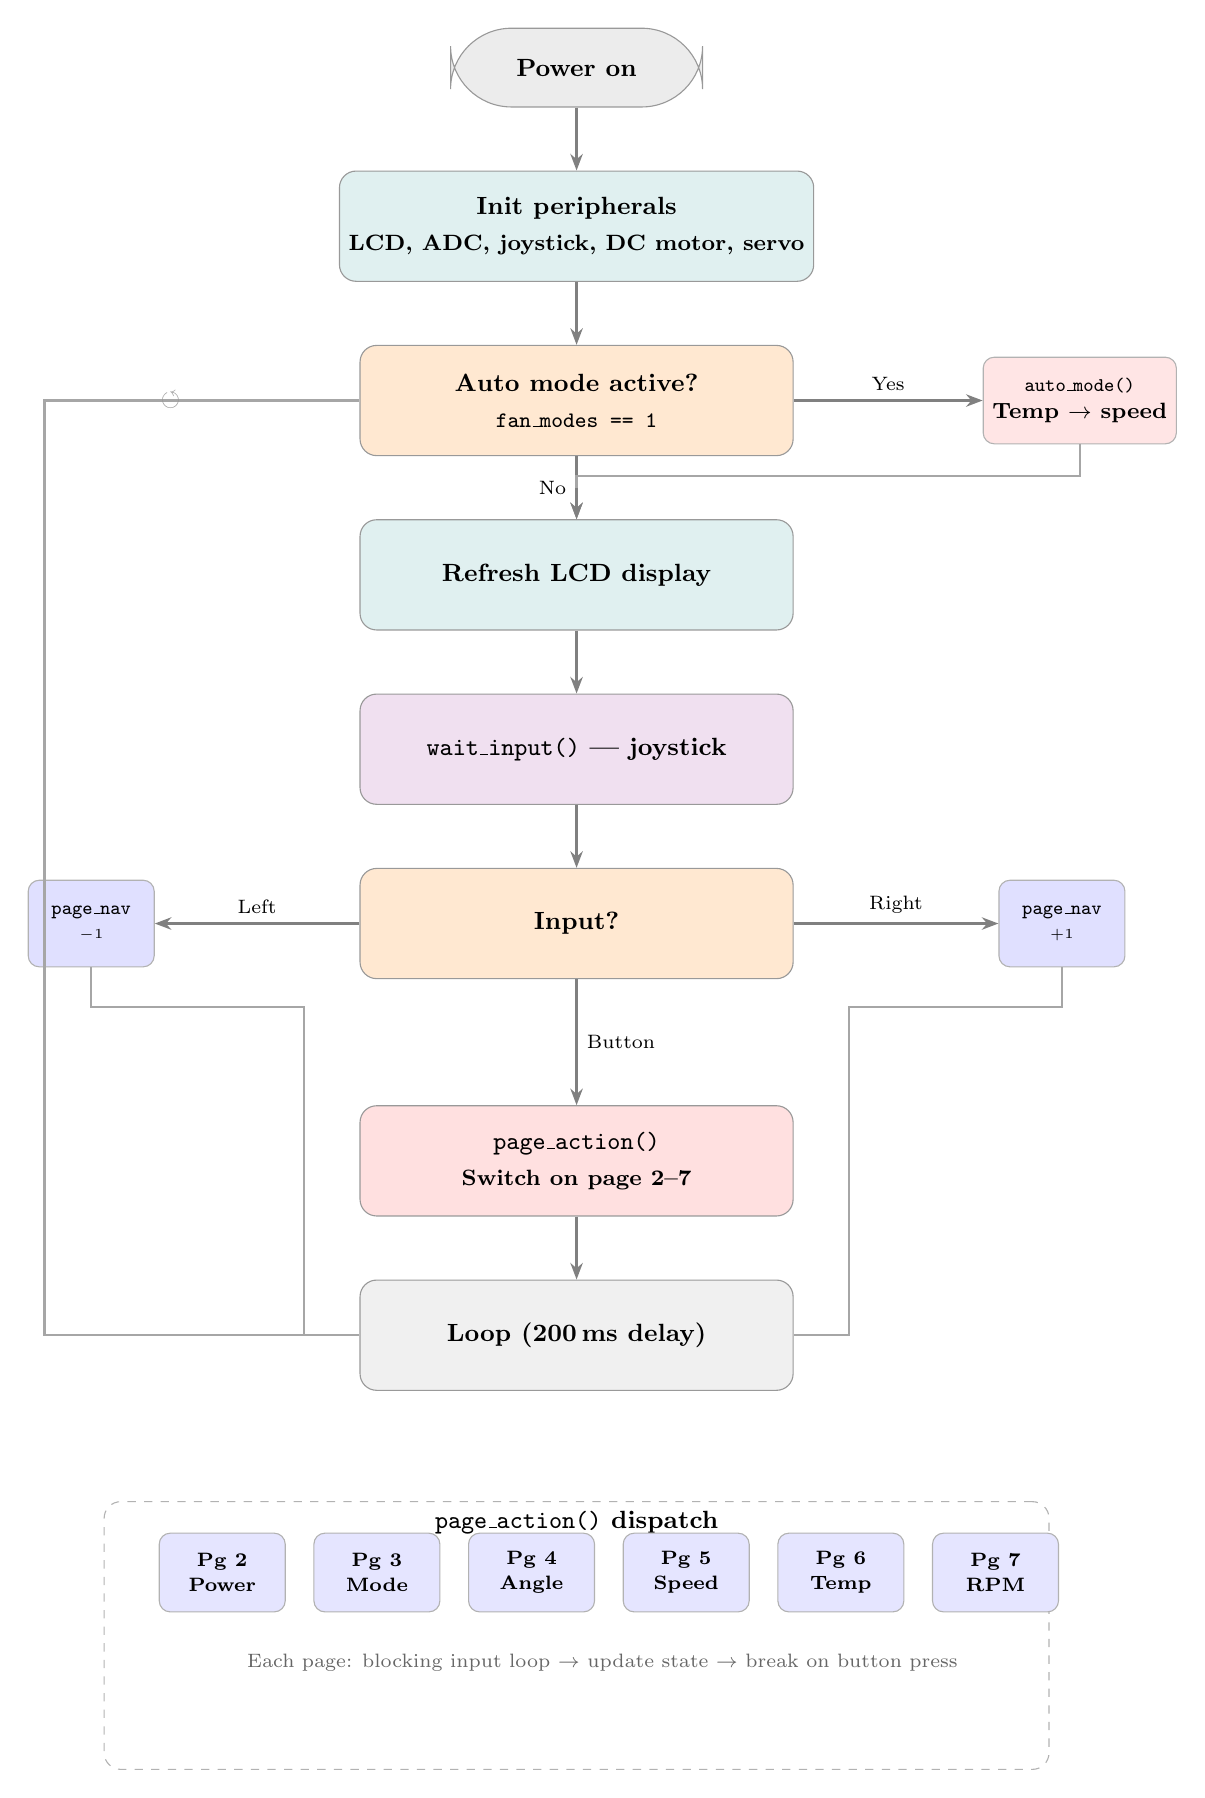
\begin{tikzpicture}[node distance=0.8cm and 2.0cm]

\node (start) [startstop]
  {Power on};

\node (init) [process, below=of start]
  {Init peripherals\\[2pt]
   {\footnotesize LCD, ADC, joystick, DC motor, servo}};

\node (autoq) [decision, below=of init]
  {Auto mode active?\\[2pt]
   {\footnotesize \texttt{fan\_modes == 1}}};

\node (lcd) [process, below=of autoq]
  {Refresh LCD display};

\node (waitin) [process, below=of lcd, fill=violet!12]
  {\texttt{wait\_input()} --- joystick};

\node (inputq) [decision, below=of waitin]
  {Input?};

\node (paction) [action, below=1.6cm of inputq]
  {\texttt{page\_action()}\\[2pt]
   {\footnotesize Switch on page 2--7}};

\node (loopend) [process, below=of paction, fill=gray!12]
  {Loop (200\,ms delay)};

\node (autoact) [sideaction, right=2.4cm of autoq]
  {\texttt{auto\_mode()}\\[2pt]
   {\footnotesize Temp $\to$ speed}};

\node (navl) [sidenote, left=2.6cm of inputq]
  {\texttt{page\_nav}\\[1pt] {\tiny $-1$}};

\node (navr) [sidenote, right=2.6cm of inputq]
  {\texttt{page\_nav}\\[1pt] {\tiny $+1$}};

%--- Main spine ---
\draw[arr] (start)   -- (init);
\draw[arr] (init)    -- (autoq);
\draw[arr] (autoq)   -- node[left,  font=\scriptsize]{No} (lcd);
\draw[arr] (lcd)     -- (waitin);
\draw[arr] (waitin)  -- (inputq);
\draw[arr] (inputq)  -- node[right, font=\scriptsize]{Button} (paction);
\draw[arr] (paction) -- (loopend);

%--- Auto mode branch ---
\draw[arr] (autoq.east) -- node[above, font=\scriptsize]{Yes} (autoact.west);
\draw[loopline] (autoact.south) -- ++(0,-0.4) -| ($(lcd.north)+(0,0.4)$);
\draw[arr] ($(lcd.north)+(0,0.4)$) -- (lcd.north);

%--- Left/Right nav ---
\draw[arr] (inputq.west) -- node[above, font=\scriptsize]{Left}  (navl.east);
\draw[loopline] (navl.south) -- ++(0,-0.5) -| ($(loopend.west)+(-0.7,0)$) -- (loopend.west);

\draw[arr] (inputq.east) -- node[above, font=\scriptsize]{Right} (navr.west);
\draw[loopline] (navr.south) -- ++(0,-0.5) -| ($(loopend.east)+(0.7,0)$) -- (loopend.east);

%--- Loop-back ---
\draw[loopline] (loopend.west) -- ++(-4.0,0) |- (autoq.west);
\node[font=\small, text=black!40] at ($(autoq.west)+(-2.4,0)$) {$\circlearrowleft$};

%--- Page dispatch legend ---
\node (leg) [draw=black!30, dashed, rounded corners=6pt,
             below=1.4cm of loopend,
             minimum width=12cm, minimum height=3.4cm,
             label={[font=\small\bfseries, anchor=north]north:\texttt{page\_action()} dispatch}] {};

\node (p2) [pagebox, below=1.8cm of loopend, xshift=-4.5cm] {Pg 2\\[1pt] Power};
\node (p3) [pagebox, right=0.35cm of p2]  {Pg 3\\[1pt] Mode};
\node (p4) [pagebox, right=0.35cm of p3]  {Pg 4\\[1pt] Angle};
\node (p5) [pagebox, right=0.35cm of p4]  {Pg 5\\[1pt] Speed};
\node (p6) [pagebox, right=0.35cm of p5]  {Pg 6\\[1pt] Temp};
\node (p7) [pagebox, right=0.35cm of p6]  {Pg 7\\[1pt] RPM};

\node[font=\scriptsize, text=black!60, below=0.4cm of p4, xshift=0.9cm]
  {Each page: blocking input loop $\to$ update state $\to$ break on button press};

\end{tikzpicture}
\end{document}